\exercice*

Considereu el trinomi de segon grau $f: x\mapsto (( a|facteur("X") )) (( b|facteur("*sox") )) (( c|facteur("so") ))$.

\begin{enumerate}
\item
\begin{enumerate}
    \item Si $x\in\mathbb{R}$. Aleshores :
        \begin{align*}
            (( a|facteur )) \,\left( x (( -x1|facteur("so") )) \right) \, \left( x (( -x2|facteur("so") )) \right)
            &= (( a|facteur )) \,\left(x\times{} x (( -x1|facteur("so") ))\times{} x (( -x2|facteur("so") ))\times{} x (( -x1|facteur("so") ))\times{} (( -x2|facteur("p") )) \right) \\
            &= (( a|facteur )) \,\left(x^2 (( (-x1-x2)|facteur("so*x") )) (( (x1*x2)|facteur("so*") ))\right) \\
            &= (( a|facteur ))\times{} x^2 (( a|facteur("so") ))\times{} (( (-x1-x2)|facteur("p*x") )) (( a|facteur("so") ))\times{} (( (x1*x2)|facteur("p") )) \\
            &= (( a|facteur("X") )) (( b|facteur("so*x") )) (( c|facteur("so") ))\\
            &= f\,(x)
        \end{align*}
    \item Si $x\in\mathbb{R}$. Aleshores :
        \begin{align*}
            (( a|facteur ))\,\left( x (( -alpha|facteur("so") )) \right)^2 (( beta|facteur("so") ))
            &= (( a|facteur ))\,\left( x^2 (( (-signealpha*2)|facteur("so") ))\times{} (( absalpha|facteur )) \times{} x + (( absalpha|facteur ))^2\right) (( beta|facteur("so") ))\\
            &= (( a|facteur ))\,\left( x^2 (( (-alpha*2)|facteur("so*x") )) + (( (absalpha**2)|facteur ))\right) (( beta|facteur("so") ))\\
            &=  (( a|facteur ))\times{} x^2 (( a|facteur("so") ))\times{} (( (-alpha*2)|facteur("p*x") )) (( a|facteur("so") ))\times{} (( (absalpha**2)|facteur )) (( beta|facteur("so") ))\\
            &= (( a|facteur("X") )) (( b|facteur("so*x") )) (( (a*absalpha**2)|facteur("so") )) (( beta|facteur("so") ))\\
            &= (( a|facteur("X") )) (( b|facteur("so*x") )) (( c|facteur("so") ))\\
            &= f\,(x)
        \end{align*}
\end{enumerate}
\item Resoleu les equacions següents triant la forma apropiada de $f$.
\begin{enumerate}
\item Si s'utilitza la forma factorizada, l'equació $f\,(x)=0$ és equivalent a l'equació del producte zero $(( a|facteur ))\,(x (( -x1|facteur("so") )) )\,(x (( -x2|facteur("so") )) ) = 0$. Així doncs :
\begin{align*}
x (( -x1|facteur("so") ))=0 &\text{ ou } x (( -x2|facteur("so") ))=0 \\
x=(( x1|facteur )) &\text{ o } x=(( x2|facteur ))
\end{align*}
Hi ha , doncs, dues solucions : $(( x1|facteur ))$ i $(( x2|facteur ))$.
\item $f\,(x)=(( c|facteur ))$ Cal remarcar que la forma desenvolupada conté la constant $(( c|facteur ))$ : aquestes haurien d'anul·lar-se, per simplificar la resolució.
\begin{align*}
f\,(x) &= (( c|facteur )) \\
(( a|facteur("X") )) (( b|facteur("so*x") )) (( c|facteur("so") )) &= (( c|facteur )) \\
(( a|facteur("X") )) (( b|facteur("so*x") )) (( c|facteur("so") )) (( -c|facteur("so") )) &= (( c|facteur )) (( -c|facteur("so") )) \\
(( a|facteur("X") )) (( b|facteur("so*x") )) &= 0 \\
\end{align*}
Ara es pot factoritzar el membre de la part esquerra en $x$, i s'obté una equació de producte zero.
\begin{align*}
(( a|facteur("X") )) (( b|facteur("so*x") )) &= 0 \\
(( a|facteur("x") ))\times{} x (( b|facteur("so") ))\times{} x &= 0 \\
x\,\left( (( a|facteur("x") )) (( b|facteur("so") )) \right) &= 0 \\
\end{align*}
\begin{align*}
x =0 &\text{ ou } (( a|facteur("x") )) (( b|facteur("so") ))=0 \\
x =0 &\text{ ou } (( a|facteur("x") )) =(( -b|facteur )) \\
x =0 &\text{ ou } x = \frac{(( -b|facteur ))}{(( a|facteur ))} \\
x =0 &\text{ ou } x = (( -(b/a)|facteur )) \\
\end{align*}
Hi ha dues solucions : $x=0$ i $x=(( -(b/a)|facteur ))$.
\item $f\,(x)=(( beta|facteur ))$ Hem de destacar que la forma canònica conté la constant $(( beta|facteur ))$ : Si s'utilitza, s'haurien de simplificar.
\begin{align*}
f\,(x) &= (( beta|facteur)) \\
(( a|facteur )) \,\left( x (( -alpha|facteur("so") )) \right)^2 (( beta|facteur("so") )) &= (( beta|facteur ))\\
(( a|facteur )) \,\left( x (( -alpha|facteur("so") )) \right)^2 (( beta|facteur("so") )) (( -beta|facteur("so") )) &= (( beta|facteur )) (( -beta|facteur("so") ))\\
(( a|facteur )) \,\left( x (( -alpha|facteur("so") )) \right)^2 &= 0\\
\left( x (( -alpha|facteur("so") )) \right)^2 &= 0\\
\end{align*}
$0$ és l'únic nombre el quadrat del qual és zero, de manera que l'equació anterior és equivalent a:
\begin{align*}
x (( -alpha|facteur("so") )) &= 0\\
x &= (( alpha|facteur )) \\
\end{align*}
Hi ha una única solució $x=(( alpha|facteur ))$.
\end{enumerate}
\item
\begin{enumerate}
\item \emph{Empleneu la taula de variacions de $f$.} En la forma desenvolupada, el coeficient davant de $x^2$ és 
(* if a > 0 *) positiu (* else *) negatiu (* endif *),
de manera que la funció és 
(* if a > 0 *) decreixent després creixent (* else *) creixent després decreixent (* endif *).
A més, l'abscissa del vèrtex és $-\frac{(( b|facteur ))}{2\times{}(( a|facteur("p") ))}$, si $(( alpha|facteur ))$, i
$f\,( (( alpha|facteur )) )=(( a|facteur ))\times{}(( alpha|facteur("p") ))^2 (( b|facteur("so") ))\times{} (( alpha|facteur("p") )) (( c|facteur("so") ))=(( beta|facteur ))$.
La taula de variacions és :
\begin{center}
    \begin{tikzpicture}
      \tkzTabInit[espcl=2.5]
      {$x$/1, $f\,(x)$/1.5}
      {$-\infty$, $(( alpha|facteur ))$, $+\infty$}
      (* if a > 0 *)
      \tkzTabVar{+/, -/$(( beta|facteur ))$/, +/}
      (* else *)
      \tkzTabVar{-/, +/$(( beta|facteur ))$/, -/}
      (* endif *)
    \end{tikzpicture}
\end{center}
\item \emph{Elaboreu la taula de signes de $f$.} Construïu una taula de signes utilizant la forma factoritzada $f\,(x)=(( a|facteur )) \,\left(x (( -x1|facteur("so") ))\right) \, \left(x (( -x2|facteur("so") ))\right)$.

\begin{itemize}
\item El primer factor $x (( -x1|facteur("so") ))$ és una funció afí, de coefficient directe $a=1$ positiu, i ordenada en l'origen $b=(( -x1|facteur ))$. És aleshores negativa, després positiva, i canvia de signe en $-\frac{b}{a}=-\frac{(( -x1|facteur ))}{1}=(( x1|facteur ))$.
\item El segon factor $x (( -x2|facteur("so") ))$ és també una funció afí, de coeficient directe $a=1$ positiu, i ordenada en l'origen $b=(( -x2|facteur ))$. És aleshores negativa, després positiva, i canvia de signe en $-\frac{b}{a}=-\frac{(( -x2|facteur ))}{1}=(( x2|facteur ))$.
\end{itemize}
\begin{center}
    \begin{tikzpicture}
      \tkzTabInit[lgt=4, espcl=2.5]
      {
        $x$/1,
        $(( a|facteur ))$/1,
        $x (( -x1|facteur("so") ))$/1,
        $x (( -x2|facteur("so") ))$/1,
        $f\,(x)=(( a|facteur ))\,\left( x (( -x1|facteur("so") )) \right)\,\left( x (( -x2|facteur("so") )) \right)$/1.5
      }
      {$-\infty$, $(( (x1, x2)|min|facteur ))$, $(( (x1, x2)|max|facteur ))$, $+\infty$}
      \tkzTabLine{, (( a|signe )), t, (( a|signe )), t, (( a|signe ))}
      (* if x1 < x2 *)
      \tkzTabLine{, -, z, +, t, +}
      \tkzTabLine{, -, t, -, z, +}
      (* else *)
      \tkzTabLine{, -, t, -, z, +}
      \tkzTabLine{, -, z, +, t, +}
      (* endif *)
      \tkzTabLine{, (( a|signe )), z, (( -a|signe )), z, (( a|signe ))}
    \end{tikzpicture}
\end{center}
\end{enumerate}
\item Contesteu les següents preguntes utilizant la taula de signes o la de variacions.
\begin{enumerate}
\item \emph{Resoleu $f\,(x)\geqslant0$.} Si s'observa l'última línia de la taula de signes es pot veure que $f$ és positiva en
(* if a > 0 *) els primers i els últims intervals (* else *) l'interval central (* endif *).
Les solucions són :
(* if a > 0 *)
   \[ x\in\interval[open left, scaled]{-\infty}{(( (x1, x2)|min|facteur ))} \cup \interval[open right, scaled]{(( (x1, x2)|max|facteur ))}{+\infty} \]
(* else *)
   \[ x\in\interval[scaled]{(( (x1, x2)|min|facteur ))}{(( (x1, x2)|max|facteur ))} \]
(* endif *)
\item \emph{ Quin és l'extrem de $f$ ?  És un màxim o un mínim ?  En quin valor de $x$ s'aconsegueix ?} En la taula de variacions s'observa que el valor més
(* if a > 0 *) xicotet (* else *) gran (* endif *)
per a $f$ és $(( beta|facteur ))$. El
(* if a > 0 *) mínim (* else *) màxim (* endif *)
de $f$ és doncs $(( beta|facteur ))$, i és aconseguit per $x=(( alpha|facteur ))$.
\end{enumerate}
\end{enumerate}
